\documentclass[11pt, a4paper, USenglish]{article} % change ``USenglish'' to ``norsk'' if applicable.

% Search http://ctan.org or type texdoc <package name> in a terminal to access LaTeX package documentation.
\usepackage{babel} % babel and csquotes are packages for multilingual (e.g. Norwegian) support.
\usepackage[T1]{fontenc} % See http://tex.stackexchange.com/questions/664/why-should-i-use-usepackaget1fontenc
\usepackage[utf8]{inputenc} % See http://tex.stackexchange.com/questions/44694/fontenc-vs-inputenc
\usepackage{csquotes} % Needs to be loaded after inputenc.
\usepackage{amsmath} % See: http://tex.stackexchange.com/questions/32100/what-does-each-ams-package-do
\usepackage{amssymb} % See above.
\usepackage[squaren]{SIunits} % Provides SI units like \meter. The squaren option is due to a conflict with amssymb.
\usepackage{graphicx} % Provides the \includegraphics command.
\usepackage{booktabs} % Better tables. Provides \toprule, \midrule, \bottomrule.
\usepackage{listings} % Provides source code listings.
\usepackage{todonotes} % Provides several handy TODO commands.
\usepackage[
  backend=bibtex,
  style=numeric,
  isbn=false,
  doi=false]{biblatex} % http://tex.stackexchange.com/questions/25701/bibtex-vs-biber-and-biblatex-vs-natbib
\usepackage{hyperref} % Provides clickable links. Always load last, but before cleveref.
\usepackage{cleveref} % Provides the \Cref command, for cross-referencing of equations, sections, figures and tables. Always load last.

\addbibresource{bibliography.bib} % Makes the bibliography file available to biblatex.

% ``listings'' package settings
\definecolor{dkgreen}{rgb}{0,0.6,0}
\definecolor{gray}{rgb}{0.5,0.5,0.5}
\definecolor{pink}{rgb}{0.63, 0.13, 0.94}
\lstset{language=Matlab, 
	keywords={break, case, catch, continue,else,elseif,end,for,function,
		global,if,otherwise,persistent,return,switch,try,while},
	basicstyle=\ttfamily,
	keywordstyle=\color{blue},
	commentstyle=\color{dkgreen},
	stringstyle=\color{pink},
	numbers=left,
	numberstyle=\tiny\color{gray},
	stepnumber=1,
	numbersep=10pt,
	backgroundcolor=\color{white},
	tabsize=4,
	showspaces=false,
        showstringspaces=false}
 % The preamble specifies all included packages and related parameters.
% \input simply inserts the contents of the file, while \include forces a \newpage.
% See \input vs. \include: http://tex.stackexchange.com/questions/246/when-should-i-use-input-vs-include

\begin{document}

% Titlepage
\title{LaTeX Lab Report Template}
\author{Group 00\\Student 70000\\Student 70001\\Student 70002}
\date{January 1, 1970}
\begin{titlepage}
    \maketitle
    \begin{figure}
    \centering
    
\includegraphics[width=0.5\textwidth]{figures/itk_ntnu}\\
    Department of Engineering Cybernetics
    \end{figure}
    \thispagestyle{empty}
\end{titlepage}

% Abstract
\newpage
\begin{abstract} 
%\addcontentsline{toc}{section}{Abstract} % add this if you want the abstract in the table of contents.
This document outlines a few important aspects of a lab report. It contains some advice on both content and layout. The \LaTeX{} source for this document is also published, and you can use it as a template of sorts for your own report. The main file, ``labreport.tex'', defines the structure of the document. The ``preamble.tex'' file is the document preamble, and contains a lot of informative comments.

When you write your own report, this section (the abstract) should contain a \emph{very} short summary of what the lab is about and what you have done.
\end{abstract}

\thispagestyle{empty} % Avoid page numbering on the abstract page.

% TOC
\newpage
\tableofcontents
\thispagestyle{empty} % Avoid page numbering on the table of contents.

% Main content
\newpage
\setcounter{page}{1}
\section{Introduction}\label{sec:intro}
Your introduction should contain an overview of the work you were assigned, as well as a few sentences putting the work into a larger perspective. You should also give a quick description of how the report is organized (as is done below).

You should of course put most of the work into doing good work in the lab and then presenting it in the report. When presenting your work in the report, both content and presentation/layout matters. Since your only way of communicating your good effort in the lab is through writing about it here, the way you write about it is essential. This means that even if you have the very best controller but describe it poorly, you will probably not be rewarded for the good results. A plot showing perfect control is worth very little if it is not accompanied by a clear description of what it represents.

Layout is naturally less important than content, but it still matters. You can think of report writing like selling an apartment; when you present your apartment for potential buyers you will of course clean the apartment and make it good looking. How clean the apartment is does of course not determine its value, but it is still important since it influences the subjective value your buyers will put on the apartment. 

\subsection{Software}
You are of course free to use whatever software you want for report writing. You can also submit a handwritten report, although this is probably not a great idea if your handwriting can be hard to read. 

You can also use Word or a similar word processor. However, it is next to impossible to achieve decent layout with Word. The support for vector graphics (discussed later) is extremely poor, and text tends to look pretty bad (bad support for kerning and ligatures). Furthermore, math is both time consuming and difficult to input, and tends to look very ugly. In general, a report written in Word looks like a draft.

It is strongly recommended to use Latex. Unless you tweak the layout too much, your report will almost certainly look very good. Although it can take a bit of effort to get started, it is also much quicker to use than Word and similar programs. The support for math and vector graphics is also great.

If you are new to Latex, you can have a look at the source for this document to get started. You can also look at the presentation by~\cite{Berland2010} (in Norwegian) or consult~\cite{Oetiker2011}. Another good reason to learn Latex is that you probably don't want to write your master's thesis in something like Word, doing so would likely be very frustrating. Being reasonably fluent in Latex before you get that far will make your thesis work much smoother.

Some of you are probably fluent in Latex and might plan to write the report using it. Please resist the temptation (if any) to change the fonts, make super fancy headers (they are not necessary for a report like this), change the margins, change the paragraph indentation and/or spacing, and similar things.

A great tool for collaborating on Latex documents is ShareLaTeX at \url{https://www.sharelatex.com/}; if you use this you won't have to install anything on your computer. Texmaker at \url{http://www.xm1math.net/texmaker/} is a good cross-platform editor. Some people like Lyx, which is a Latex editor that behaves a little bit like Word. If you prefer to compile your Latex document on the command line, the latexmk \url{https://www.ctan.org/pkg/latexmk} command is a great tool included in most TeX distributions. There is also a simple Vim plugin that uses latexmk as its backend called LaTeX-BoX \url{https://github.com/LaTeX-Box-Team/LaTeX-Box}.

\subsection{Other Comments}
Unless you have a very good reason not to, you should write the report in English. If you have problems with Latex, the solution is usually just a few Google searches away.

This report is organized as follows: \Cref{sec:prob_descr} contains some equations relevant for TTK4135, and some tips on how to create illustrations. Several \LaTeX{} tips can be foundin \Cref{sec:latex_tips}, such as how to create a table and matrix equations. \Cref{sec:figures} contains some advice on using plots from MATLAB\@. The closing remarks are in~\Cref{sec:conclusion}, respectively. \Cref{sec:matlab} contains a MATLAB file while \Cref{sec:simulink} shows an example Simulink diagram. The Bibliography can be found at the end, on page~\pageref{sec:bibliography}.

\section{Problem Description}\label{sec:prob_descr}
You should have a section that describes the lab setup, including a model of the helicopter. If you want, you can copy the source code for the model equations:
\begin{gather}
	\ddot{e} + K_{3} K_{ed} \dot{e} + K_{3} K_{ep} e = K_{3} K_{ep} e_{c} \label{eq:model_elev} \\
	\ddot{p} + K_{1} K_{pd} \dot{p} + K_{1} K_{pp} p = K_{1} K_{pp} p_{c} \label{eq:model_pitch} \\
	\dot{\lambda} = r \label{eq:model_lambda} \\
	\dot{r} = -K_{2} p \label{eq:model_r} 
\end{gather}
Since these equations belong together, it's a good idea to number them like this:
\begin{subequations}\label{eq:model}
	\begin{gather}
		\ddot{e} + K_{3} K_{ed} \dot{e} + K_{3} K_{ep} e = K_{3} K_{ep} e_{c} \label{eq:model_se_elev} \\
		\ddot{p} + K_{1} K_{pd} \dot{p} + K_{1} K_{pp} p = K_{1} K_{pp} p_{c} \label{eq:model_se_pitch} \\
		\dot{\lambda} = r \label{eq:model_se_lambda} \\
		\dot{r} = -K_{2} p \label{eq:model_se_r} 
	\end{gather}
\end{subequations}
You can then both reference individual equations (``the elevation equation \Cref{eq:model_se_elev}'') or reference the entire model (``the linear model~\Cref{eq:model}''). Regardless of your choice of software, never hard-code a reference, always use dynamic references. 

You could also align the equations like this:
\begin{subequations}\label{eq:model_al}
	\begin{align}
		\ddot{e} + K_{3} K_{ed} \dot{e} + K_{3} K_{ep} e &= K_{3} K_{ep} e_{c} \label{eq:model_se_al_elev} \\
		\ddot{p} + K_{1} K_{pd} \dot{p} + K_{1} K_{pp} p &= K_{1} K_{pp} p_{c} \label{eq:model_se_al_pitch} \\
		\dot{\lambda} &= r \label{eq:model_se_al_lambda} \\
		\dot{r} &= -K_{2} p \label{eq:model_se_al_r} 
	\end{align}
\end{subequations}
You can consult~\cite{Downes2002} for more about writing math.


\subsection{Illustrations}
If you decide to include an illustration, that's great. You can in general copy figures and illustrations from the textbook, the assignement text, or other places. However: ALWAYS CITE THE SOURCE\@. You can also draw your own (cite the source if it is heavily based on someone else's.). \Cref{fig:layers_openloop} was created quickly with Ipe (\url{http://ipe.otfried.org/}). Inkscape is a good alternative for more advanced illustrations. Some people prefer the Latex package TikZ (\url{http://texample.net/tikz/examples/}), but this takes a little effort to learn.

\begin{figure}[tp]
	\centering
	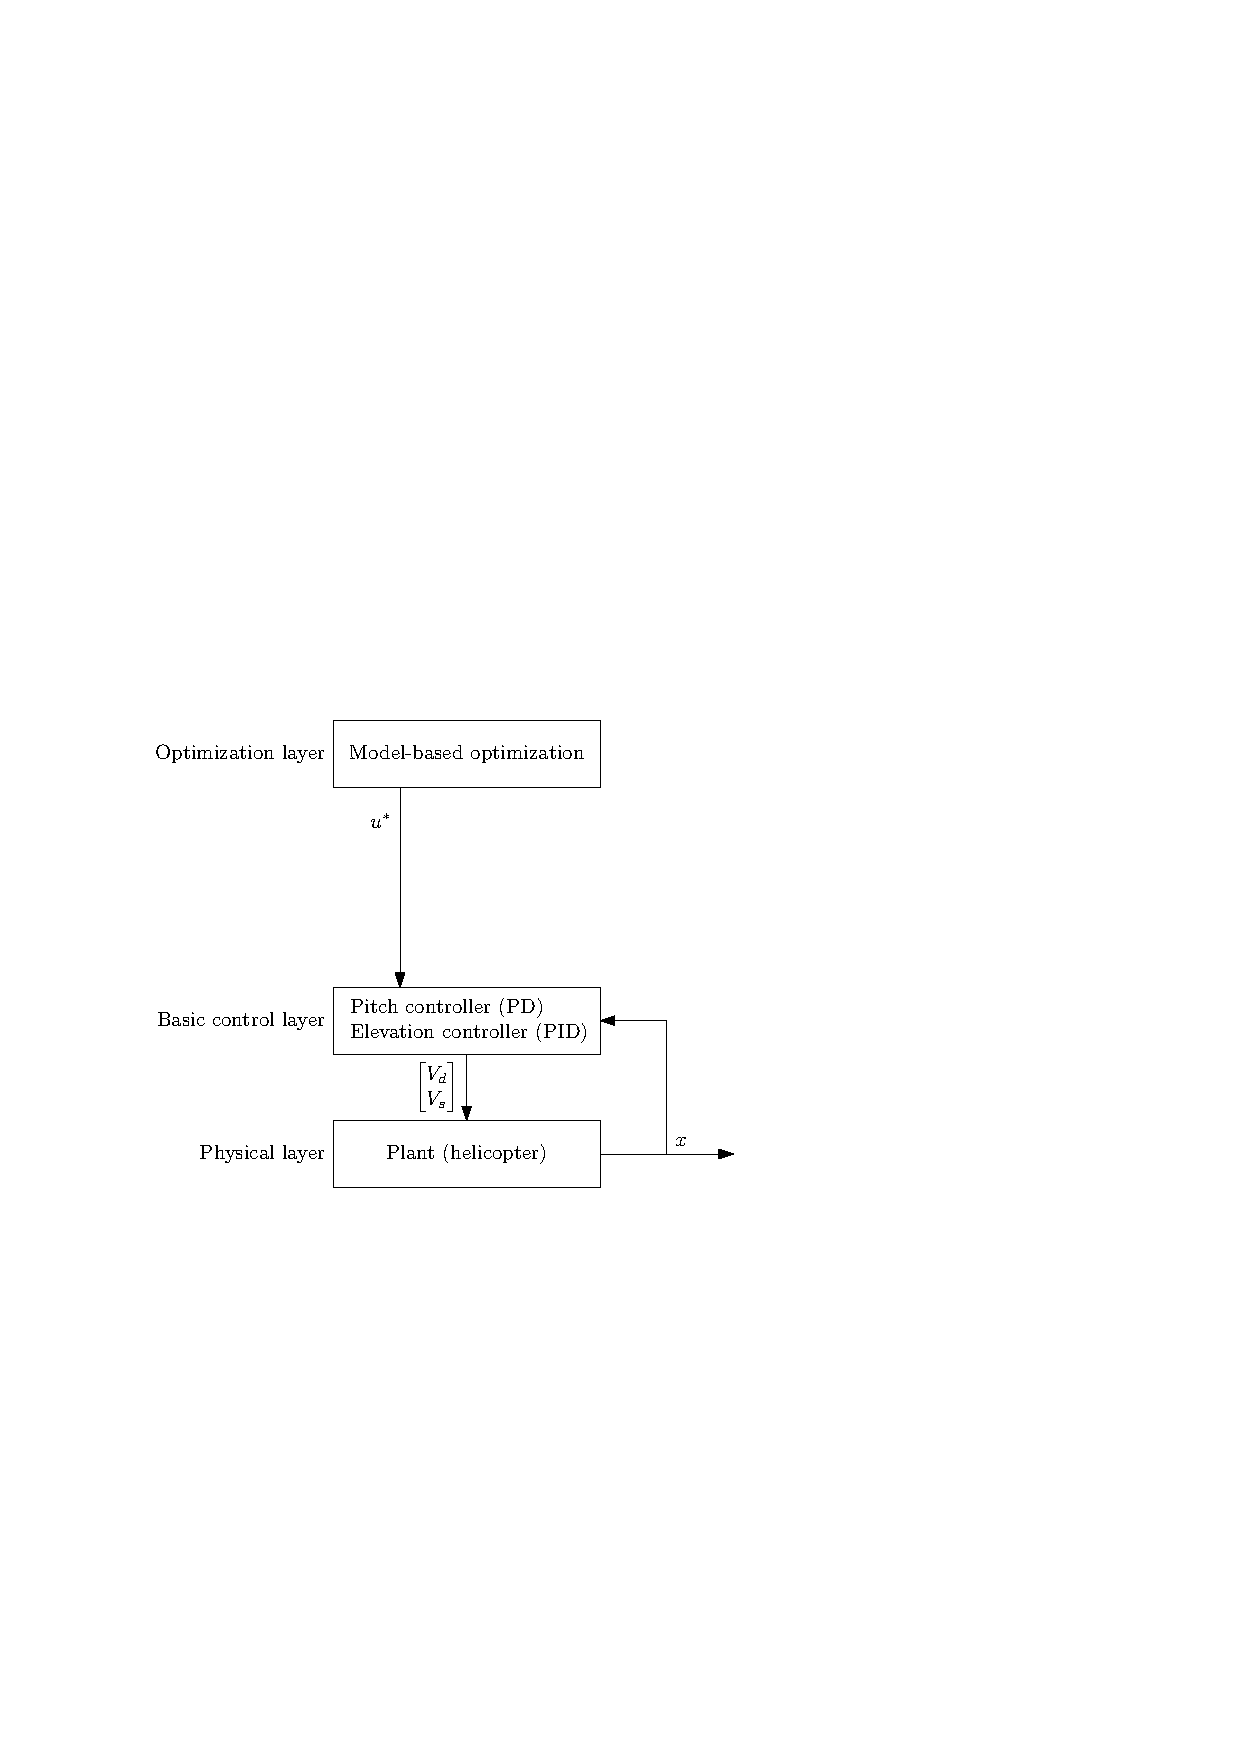
\includegraphics[width=1.00\textwidth]{figures/layers_openloop.pdf}
	\caption{A figure created with Ipe for TTK4135.}
\label{fig:layers_openloop}
\end{figure}

\newcommand{\texMacro}[2]{\texttt{\textbackslash{#1}\{#2\}}}
\section{General LaTeX tips}\label{sec:latex_tips}
Some tips were given in \Cref{sec:intro}, and this section will elaborate with some more concrete examples.

\subsection{Matrix Equations}
Here is a matrix equation you can use as a template:
\begin{equation}
	\begin{bmatrix}
		1 &  0 &  0 & 0 & -b &  0 &  0 &  0 \\
		-a &  1 &  0 & 0 &  0 & -b &  0 &  0 \\
		0 & -a &  1 & 0 &  0 &  0 & -b &  0 \\
		0 &  0 & -a & 1 &  0 &  0 &  0 & -b                                
	\end{bmatrix}
	\begin{bmatrix} x_1 \\ x_2 \\ x_3 \\ x_4 \\ u_0 \\ u_1 \\ u_2 \\ u_3 \end{bmatrix}
	=
	\begin{bmatrix}
		ax_0 \\ 0 \\ 0 \\ 0      
	\end{bmatrix}
\end{equation}

\subsection{Tables}
If you want, you can use the source for \Cref{tab:parameters} to see how a (floating) table is made. 

Variables and symbols are always in italics, while units are not.

\begin{table}[tbp]
	\centering
	\caption{Parameters and values.}
	\begin{tabular}{llll}
		\toprule
		Symbol & Parameter & Value & Unit \\
		\midrule
		$l_a$ & Distance from elevation axis to helicopter body & $0.63$ & \meter\\
		$l_h$ & Distance from pitch axis to motor & $0.18$ & \meter\\
		$K_f$ & Force constant motor & $0.25$ & \newton\per\volt\\
		$J_e$ & Moment of inertia for elevation & $0.83$ & \kilogram\usk\meter\squared\\
		$J_t$ & Moment of inertia for travel & $0.83$ & \kilogram\usk\meter\squared\\
		$J_p$ & Moment of inertia for pitch & $0.034$ & \kilogram\usk\meter\squared\\
		$m_h$ & Mass of helicopter & $1.05$ & \kilogram\\
		$m_w$ & Balance weight & $1.87$ & \kilogram\\
		$m_g$ & Effective mass of the helicopter & $0.05$ & \kilogram\\
		$K_p$ & Force to lift the helicopter from the ground & $0.49$ & \newton\\
		\bottomrule
	\end{tabular}
\label{tab:parameters}
\end{table}

\subsection{The \texMacro{input}{} command}
By using \texMacro{input}{whatever} in your main tex file (\texttt{labreport.tex} in this case), the content of \texttt{whatever.tex} will be included in your pdf. This way you can split the contents into different files, e.g.~one for each problem of the assignment. This makes it easier to restructure the document, and arguably improves the readability of the tex files. For instance; maybe you want each problem to start on a new page? Simply add \textbackslash{newpage} before each \texMacro{input}{} command. Alternatively, you can use the \texMacro{include}{} command to achieve more or less the same effect. See~\cite{InputVsInclude} for more information.

\subsection{Citations and Reference Management}
In academic writing, it is very important to cite your sources. In Latex this is done by defining an an entry in a \emph{BibTeX} bibliography file like this (from \texttt{bibliography.bib}):
\lstinputlisting[language=Tex, firstline=1, lastline=7]{bibliography.bib}
and then using the \texttt{\textbackslash{cite}} command in your Latex document. For instance \texttt{\textbackslash{cite}\{Chen2014\}} will produce~\cite{Chen2014}.

There are many different citation styles, and a lot of customization that is possible, so please check out e.g.~\cite{BiberBibtexEtc,WikibookLatex}\footnote{Keep citation of web pages to a minimum, and consider using \url{http://web.archive.org} if you are worried that the reference may change or be removed in the future.}.

There is also a lot of useful software to manage your references. Some popular examples include JabRef (\url{http://www.jabref.org/}), Mendeley (\url{https://www.mendeley.com/}) and EndNote. JabRef is perhaps the simplest of these three, and stores all information in a \texttt{.bib} file that you can directly use in your Latex document. Both Mendeley and EndNote can export references as BibTeX.

\section{Results and Figures}\label{sec:figures}
Answer all the parts of the exercise in an organized and clear manner. You should of course try to get good results in all the exercises, but if you have made a good effort without achieving great performance, a good discussion of possible reasons is just as good. Present your thinking and efforts and discuss possible reasons for good or bad results.

Include plots and/or tables of all relevant results, but make sure you don't overwhelm the reader with too many plots. Have a clear plan about what you want to communicate with a specific plot/figure, and use appropriate labels and comments. Keep in mind that the plots should be as ``readable'' as possible; that is, they should not be too hard to interpret and be reasonably self contained.

There are some important things to consider when exporting figures from MATLAB, most importantly which format you use. Never ever use JPEG for anything that is not a photography or similar. Any figure, like a plot or block diagram, must never be stored as a JPEG\@. If you zoom in on Figure~\ref{fig:constraint_jpg} you can see a lot of noise close to any of the dark curves and lines, this is due to the compression in JPEG\@. Figure~\ref{fig:constraint_jpg} will look horrible both on a screen and on paper.

The PNG format is slightly better for plots, but since it is a raster format (a grid of pixels), it looks ugly if you zoom in. It also looks ugly if you scale it, both on a screen and on paper. Try to avoid PNG if you can. Figures~\ref{fig:constraint_png} and~\ref{fig:constraint_png_large} are both PNG figures; the latter being a larger figure scaled more than the former. Note both how choppy and ugly the blue curve is, and how the different sizes create inconsistent font sizes.

The simplest way to get a reasonably good looking plot is to save it as EPS in MATLAB\@. Do this by clicking ``File'' in the figure window, and the ``Save As\ldots''; choose ``EPS file (*.eps)'' in the ``Save as type:'' menu.\footnote{pdfLatex does not support EPS directly, but since we have loaded the \emph{epstodf} package, this is not a problem.} Figure~\ref{fig:constraint_eps} shows a plot in EPS format. Since EPS is a vector format, the Figure can be scaled and still look good (but mind the font size!). If you zoom in you can see that the curve and the letters/numbers are smooth. A figure in vector format will usually look good both on a screen and on paper.

Note that the size of the actual figure window in MATLAB determines how large the exported figure is. Hence, if you enlarge the figure window before exporting, you will need to scale the figure by a larger factor in the report. This will lead to a tiny font in the figure. There are many better ways of exporting graphics from MATLAB, but they quickly become fairly involved. The above method of exporting to EPS will in most cases give nice figures.

You can write Latex in your MATLAB figures. The script used to create Figures~\ref{fig:constraint_jpg}--\ref{fig:constraint_eps} is included in Section~\ref{sec:plot_constraint_m}. Do not use a screen shot of a scope of figure in MATLAB in your report.

\begin{figure}[htb]
	\centering
		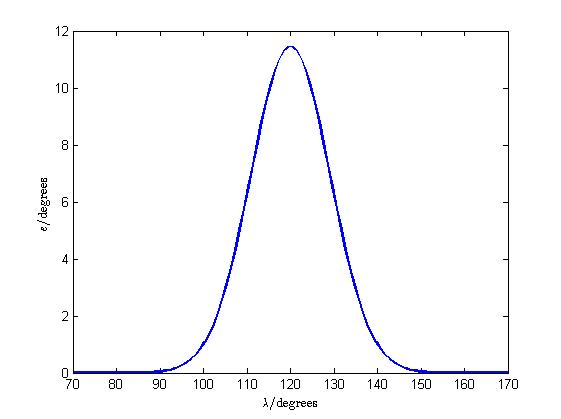
\includegraphics[width=0.8\textwidth]{figures/constraint_jpg.jpg}
	\caption{A plot in JPEG format --- a very bad idea.}
\label{fig:constraint_jpg}
\end{figure}

\begin{figure}[htb]
	\centering
		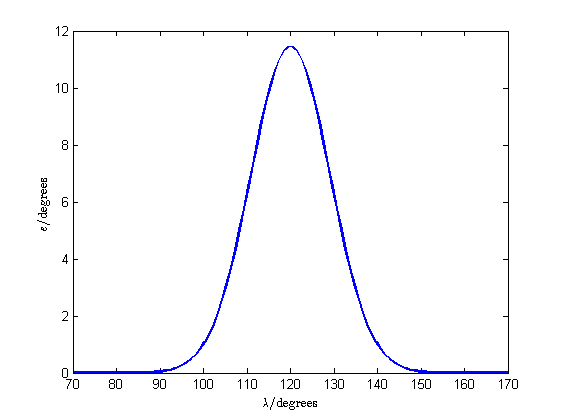
\includegraphics[width=0.8\textwidth]{figures/constraint_png.png}
	\caption{A plot in PNG format --- a bad idea.}
\label{fig:constraint_png}
\end{figure}

\begin{figure}[htb]
	\centering
		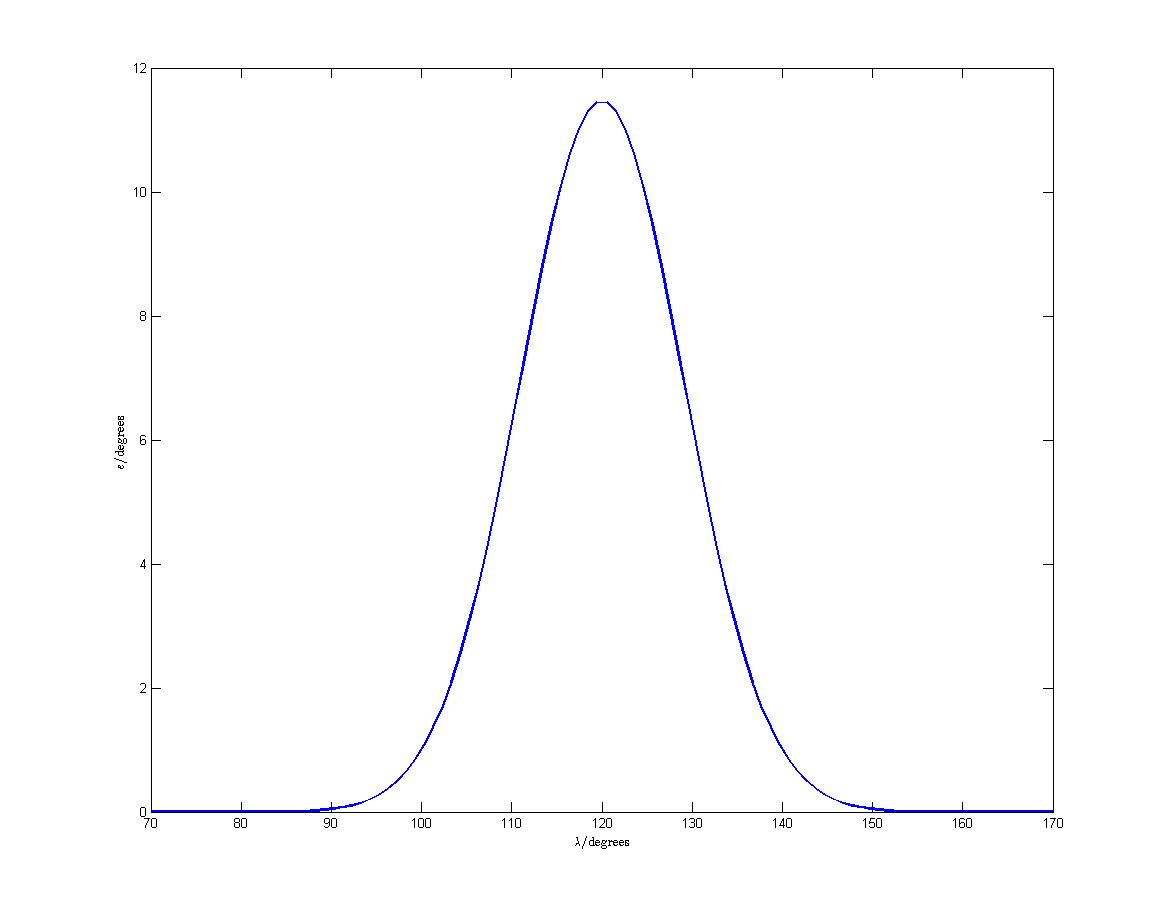
\includegraphics[width=0.8\textwidth]{figures/constraint_png_large.png}
	\caption{A plot in PNG format --- a bad idea. This figure is originally larger than the other PNG figure, but both are scaled to the same size.}
\label{fig:constraint_png_large}
\end{figure}

\begin{figure}[htb]
	\centering
		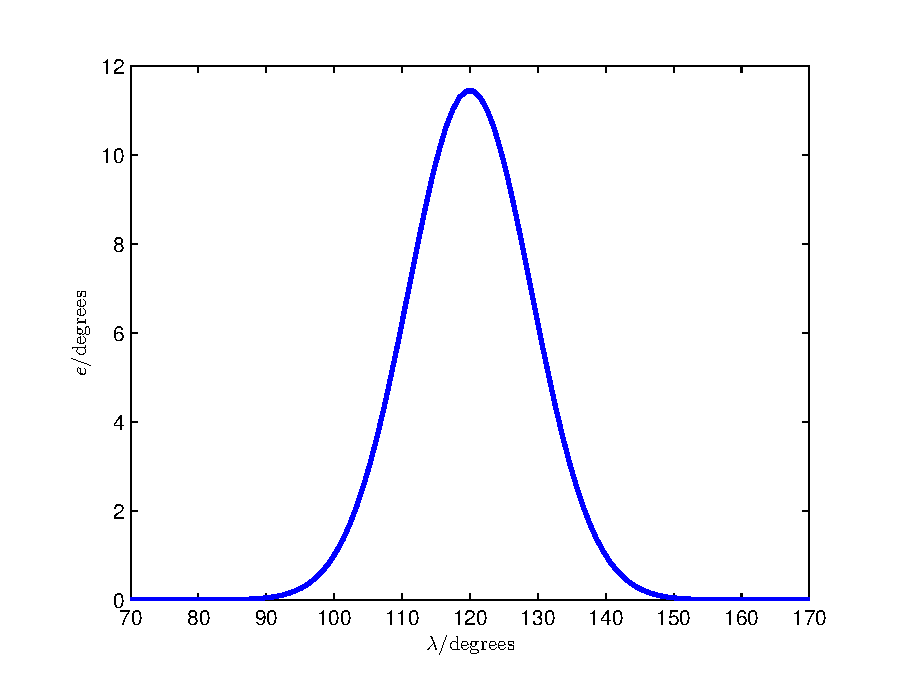
\includegraphics[width=0.8\textwidth]{figures/constraint_eps.eps}
	\caption{A plot in EPS format --- a much better idea.}
\label{fig:constraint_eps}
\end{figure}

Remember to reference all figures in the text. Figures have a number and should be referenced by that number (again, always use dynamic references). They also tend to float around, meaning they generally don't appear where you ask them to in the text. This is fine, do not try to force a figure (or a table) to appear in a particular place. As long a you refer to it, it's easy to find. No figure should be included without being referenced in the text.

If you look at the source code for including figures, you can see that the optional option \verb+[htb]+ has been used. This tells Latex where you wish the figure to appear, in prioritized order. \verb+h+ means ``Here'', t means ``Top of this page'', b means ``Bottom of this page'', and p (not used here) means ``on a Page with only floats (such as figures and tables)''. Note that your wish might not be granted, and this is because Latex actually optimizes the placement of figures. If you start forcing figures to be in specific places, it often leads to really strange layout somewhere else in the document. 

Generally, let Latex handle the documentation layout. This is one of the main reasons to choose Latex over software such as Microsoft Word.

\subsection{Results and Discussion}
All problems should have their own discussion of results. 

Remember: all plots and results need a description, explanation, and discussion.

\section{Conclusion}\label{sec:conclusion}
This does not have to be long, but try to write a few reasonable closing remarks.

\addcontentsline{toc}{section}{Appendix} % Remove this if you don't want the appendix included in the table of contents.
\appendix

\section{MATLAB Code}\label{sec:matlab}
This section should contain your MATLAB code. DO NOT attach files posted online (that you didn't write). Note that the method used to input code below does not look as pretty when the lines are too long.

\subsection{plot\_constraint.m}\label{sec:plot_constraint_m}
\lstinputlisting{code/plot_constraint.m}\section{Simulink Diagrams}\label{sec:simulink}
This section should contain your Simulink diagrams. Just like the plots, these should be in vector format, like in Figure~\ref{fig:simulink}. Make them tidy enough to understand.

\subsection{A Simulink Diagram}
Figure~\ref{fig:simulink} shows a Simulink diagram.
\begin{figure}[htb]
	\centering
		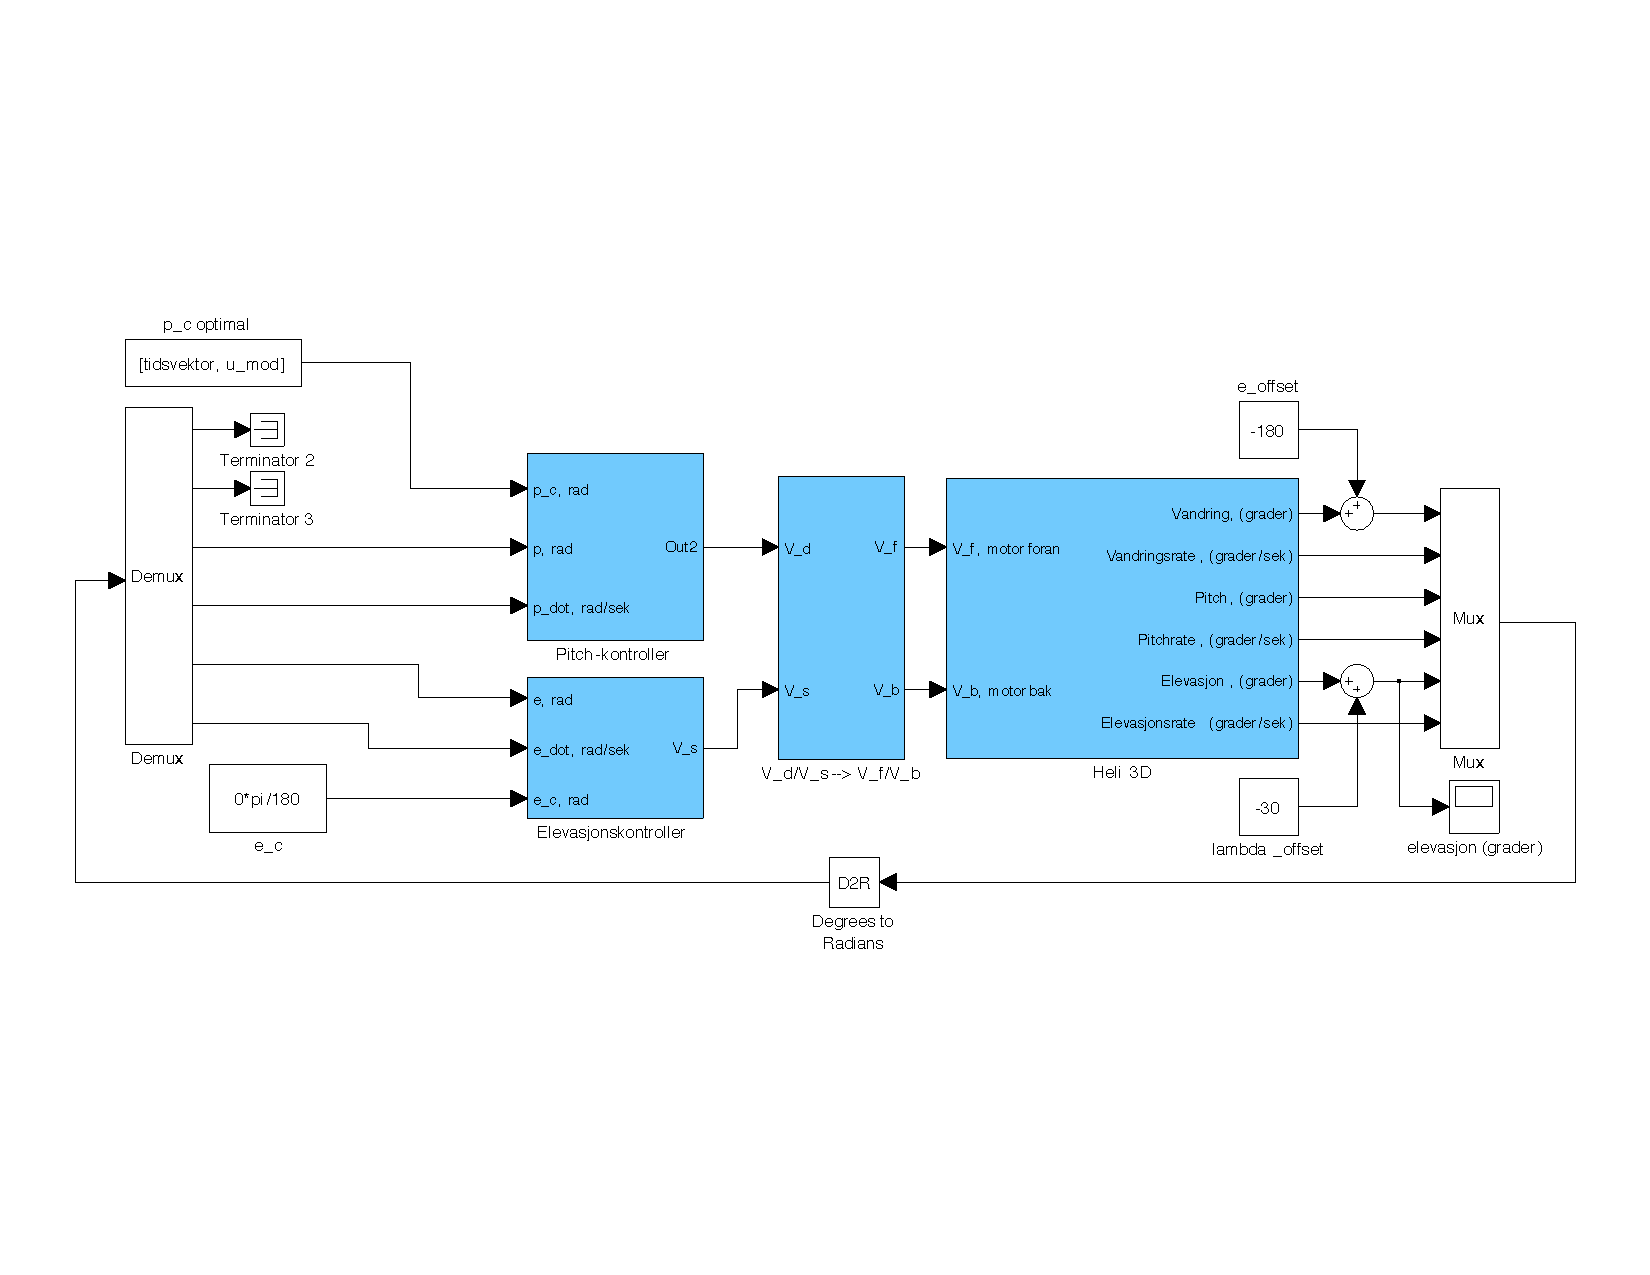
\includegraphics[width = \textwidth]{figures/simulink.pdf}
	\caption{A Simulink diagram.}
\label{fig:simulink}
\end{figure}


% References
\newpage
\addcontentsline{toc}{section}{References}
\printbibliography{}
\label{sec:bibliography}

\end{document}
